\section{Scheduling and Design}
% \begin{subbox}{Tasks}
%     \begin{enumerate}
%         \item \textbf{Project Schedule} - come up with a schedule of your overall project based on the user stories created in the previous milestones.
%         \item \textbf{Project Scheduling Tools} - which tools are you using? E.g. Pivotal Tracker, Jira
%         \item \textbf{Design of Components} - Describe different components of your system based on the user stories created in the previous milestones.
%         \item \textbf{Software Design} - Basic class diagrams of your proposed system.
%     \end{enumerate}
% \end{subbox}


\subsection{Project Schedule}
\subsubsection{Gantt Chart}
After a lot of discussion, a general schedule mentioned in \autoref{fig:complete_timeline} has been decided. The breakdown of individual milestone in \autoref{fig:complete_timeline} is given in \autoref{fig:tl_ms1_ms2}, \autoref{fig:tl_ms3_ms4} and \autoref{fig:tl_ms5_ms6}. Details about each task is given in \autoref{table:sprint_schedule}.

% \begin{table}[H]
% \centering
% \begin{tabular}{|c|c|}
% \hline
% \textbf{Milestone} & \textbf{Schedule} \\ \hline
% 1, 2               &  \autoref{fig:tl_ms1_ms2}\\ \hline
% 3, 4               &  \autoref{fig:tl_ms3_ms4}\\ \hline
% 5, 6               &   \autoref{fig:tl_ms5_ms6}\\ \hline
% \end{tabular}
% \caption{}
% \label{tab:my-table}
% \end{table}

\begin{figure}[H]
    \centering
    \fbox{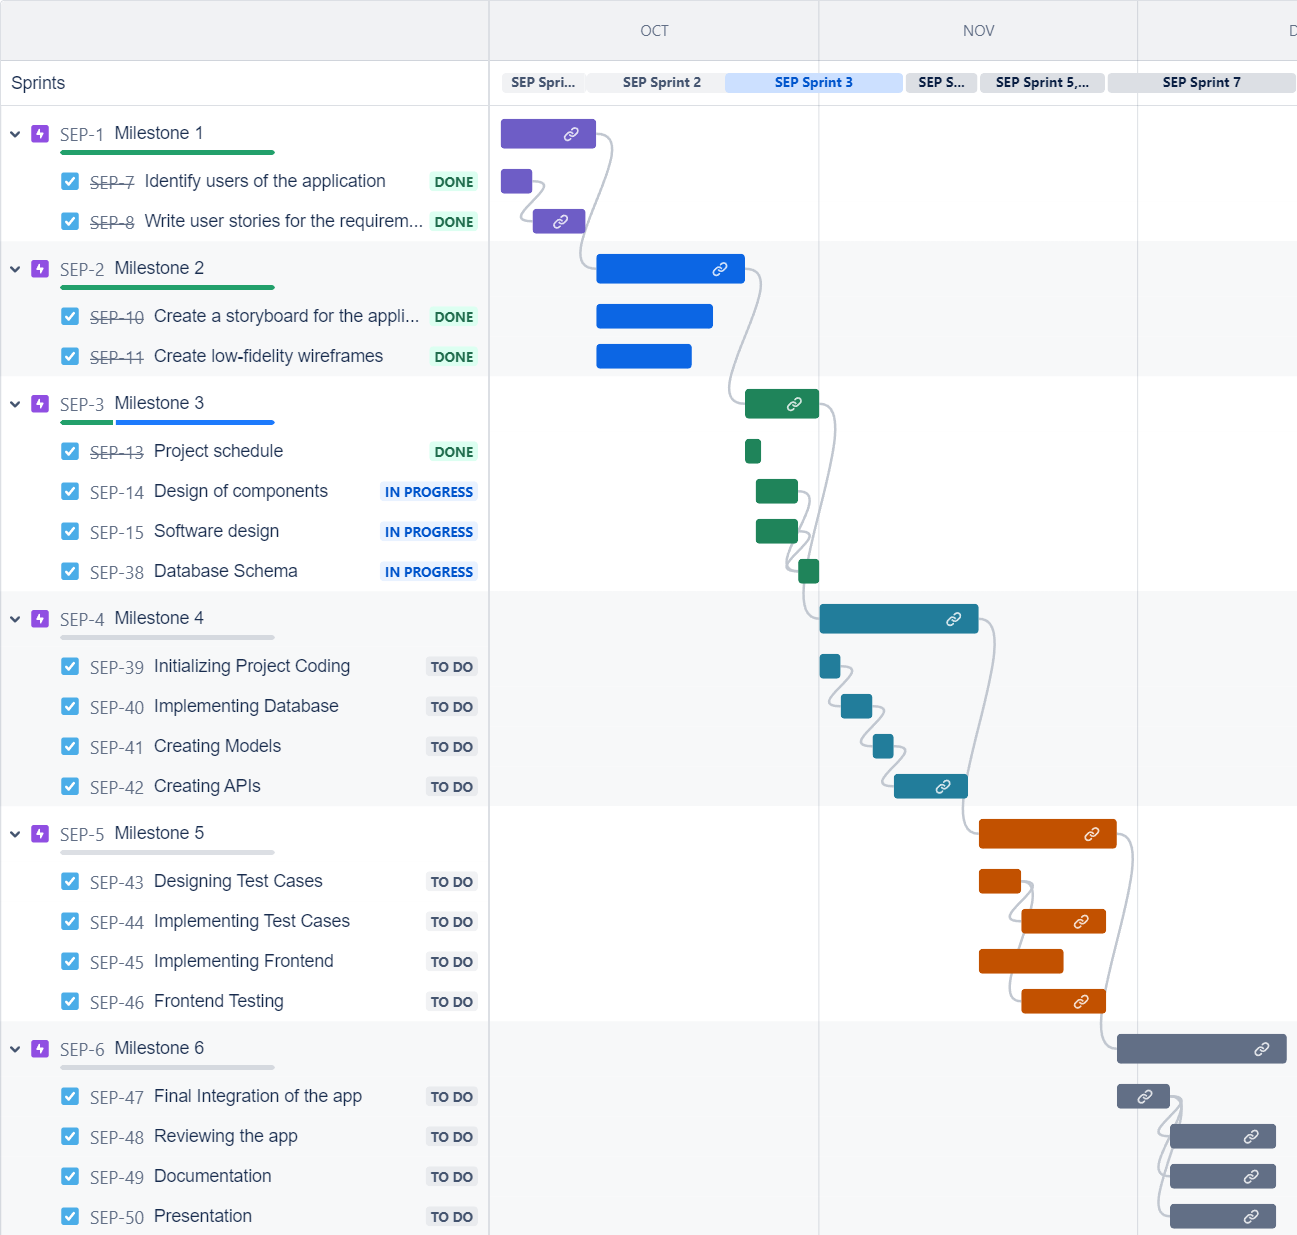
\includegraphics[width=0.95\textwidth]{img/TL_complete.png}}
    \caption{Complete Project Timeline}
    \label{fig:complete_timeline}
\end{figure}

\begin{figure}[H]
    \centering
    \fbox{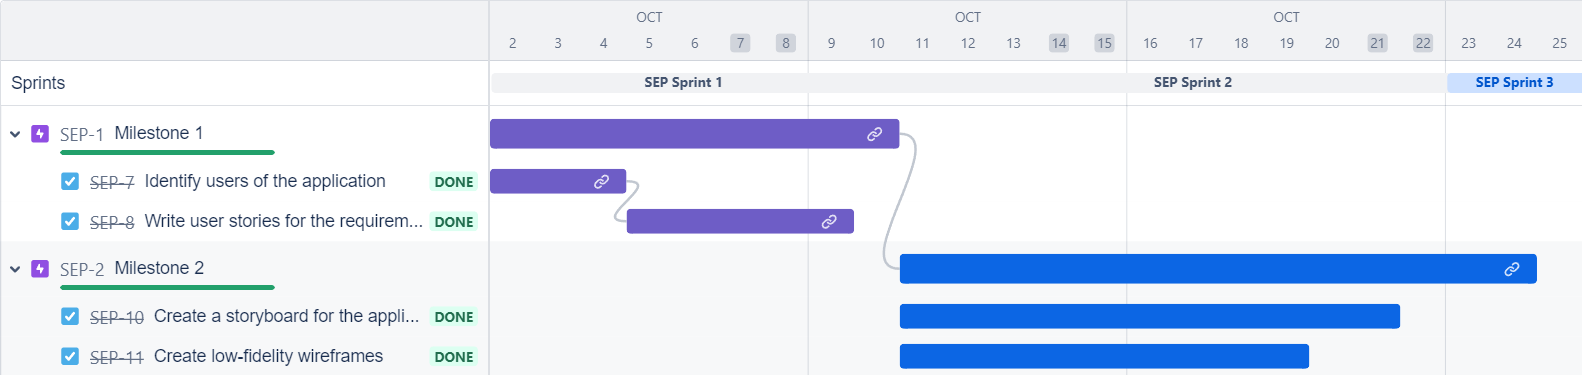
\includegraphics[width=1\textwidth]{img/TL_MS1_MS2.png}}
    \caption{Milestone 1 and 2 Schedule}
    \label{fig:tl_ms1_ms2}
\end{figure}

\begin{figure}[H]
    \centering
    \fbox{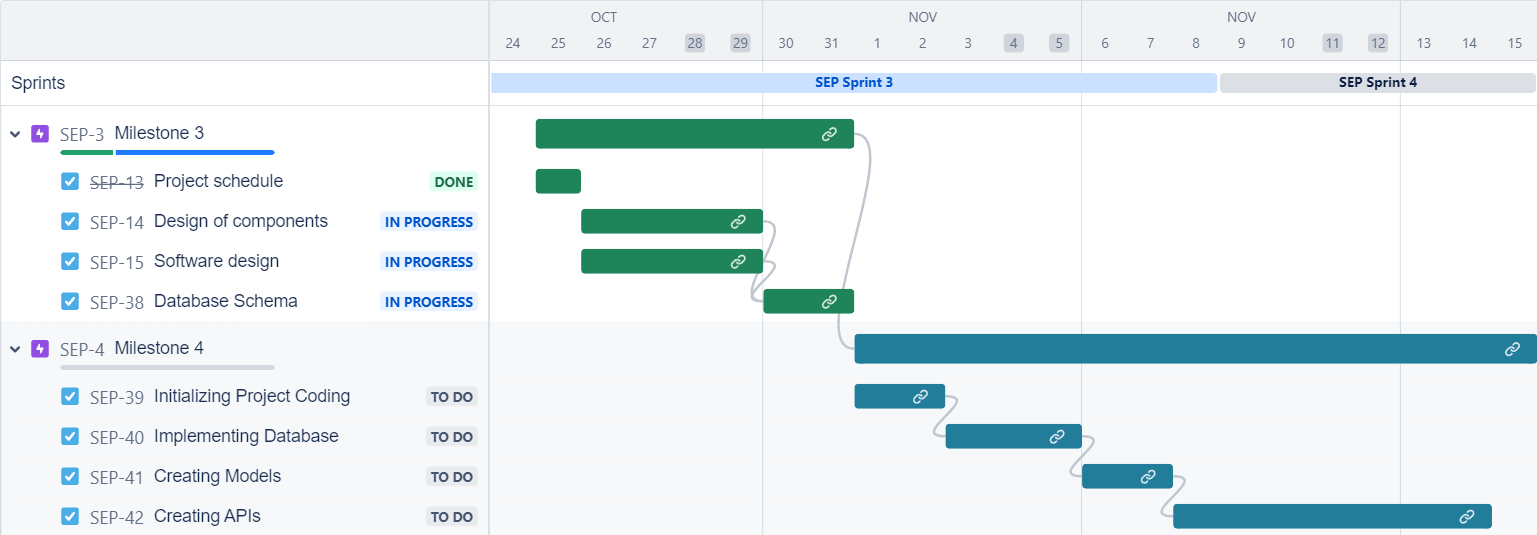
\includegraphics[width=1\textwidth]{img/TL_MS3_MS4.png}}
    \caption{Milestone 3 and 4 Schedule}
    \label{fig:tl_ms3_ms4}
\end{figure}

\begin{figure}[H]
    \centering
    \fbox{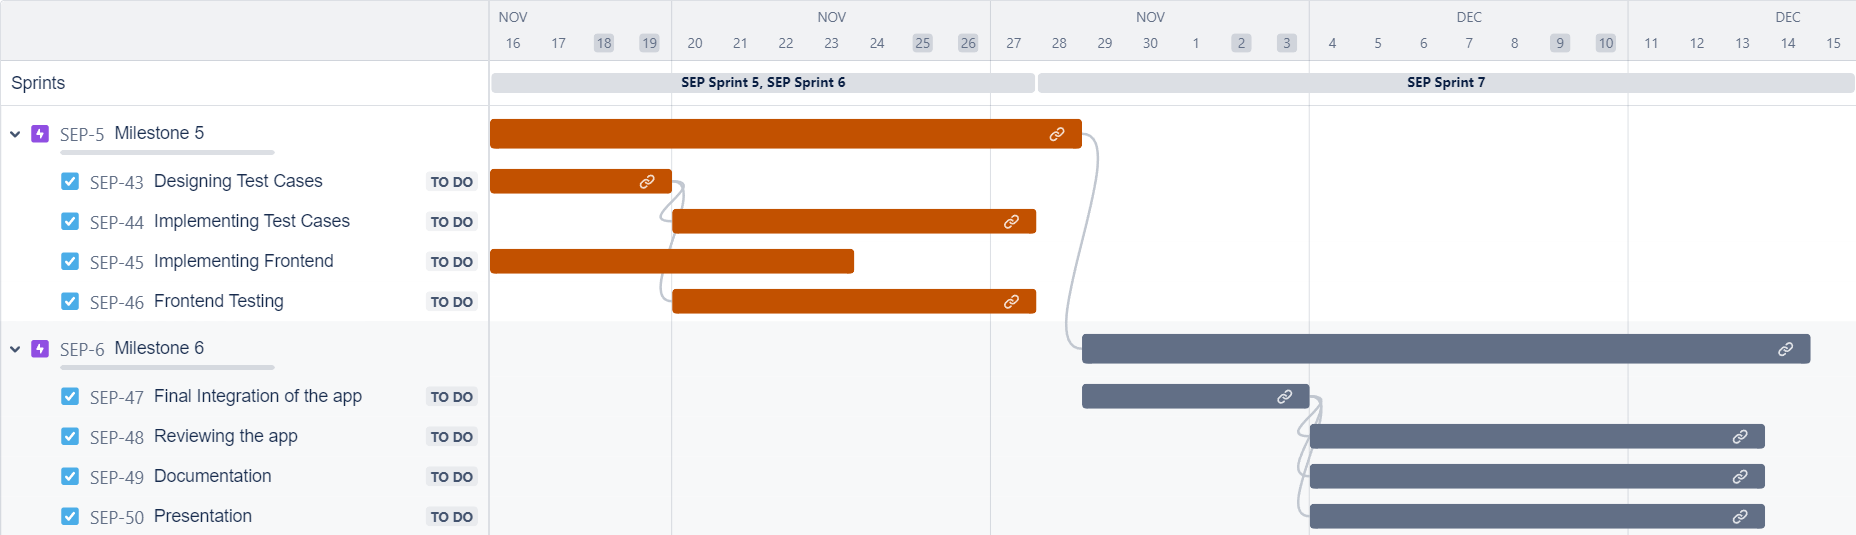
\includegraphics[width=1\textwidth]{img/TL_MS5_MS6.png}}
    \caption{Milestone 5 and 6 Schedule}
    \label{fig:tl_ms5_ms6}
\end{figure}

As evident from the figures, each task in the milestones is self-explanatory and need not be further described.

The tasks above have divided into various sprints, details of which are in \autoref{table:sprint_schedule}.

\subsubsection{SPRINT Schedule}
\begin{table}[H]
\def\arraystretch{1.5}
\begin{center}
    \begin{tabular}{|m{7cm}|m{3cm}|m{3cm}|m{3cm}|}
        \hline
        \rowcolor{heading-grey}\multicolumn{1}{|>{\centering\arraybackslash}m{70mm}|}{\textcolor{white}{\textbf{Activity}}} & 
        \multicolumn{1}{|>{\centering\arraybackslash}m{30mm}|}{\textcolor{white}{\textbf{Start Date (dd/mm/yyy)}}} & 
        \multicolumn{1}{|>{\centering\arraybackslash}m{30mm}|}{\textcolor{white}{\textbf{End Date (dd/mm/yyyy)}}} &
        \multicolumn{1}{|>{\centering\arraybackslash}m{30mm}|}{\textcolor{white}{\textbf{Duration (days)}}} \\ \hline
                
\multicolumn{4}{|l|}{\cellcolor{heading2-grey} \textbf{Sprint 1}} \\ \hline
Identify users of the application & 02/10/2023 & 04/10/2023 & 3 \\ \hline
Write user stories & 05/10/2023 & 09/10/2023 & 5 \\ \hline

\multicolumn{4}{|l|}{\cellcolor{heading2-grey} \textbf{Sprint 2}} \\ \hline
Create storyboards & 11/10/2023 & 21/10/2023 & 11 \\ \hline
Create low-fidelity wireframes & 11/10/2023 & 19/10/2023 & 9 \\ \hline

\multicolumn{4}{|l|}{\cellcolor{heading2-grey} \textbf{Sprint 3}} \\ \hline
Project schedule & 25/10/2023 & 25/10/2023 & 1 \\ \hline
Design of components & 26/10/2023 & 29/10/2023 & 4 \\ \hline
Software design & 26/10/2023 & 29/10/2023 & 4 \\ \hline
Database Schema & 30/10/2023 & 31/10/2023 & 2 \\ \hline
Initializing Project Coding & 01/11/2023 & 02/11/2023 & 2 \\ \hline
Implementing Database & 03/11/2023 & 05/11/2023 & 3 \\ \hline
Creating Models & 06/11/2023 & 07/11/2023 & 2 \\ \hline

\multicolumn{4}{|l|}{\cellcolor{heading2-grey} \textbf{Sprint 4}} \\ \hline
Creating APIs & 08/11/2023 & 14/11/2023 & 7 \\ \hline

\multicolumn{4}{|l|}{\cellcolor{heading2-grey} \textbf{Sprint 5}} \\ \hline
Designing Test Cases & 16/11/2023 & 19/11/2023 & 4 \\ \hline
Implementing Test Cases & 20/11/2023 & 27/11/2023 & 8 \\ \hline

\multicolumn{4}{|l|}{\cellcolor{heading2-grey} \textbf{Sprint 6}} \\ \hline
Implementing Frontend & 16/11/2023 & 23/11/2023 & 8 \\ \hline
Frontend Testing & 20/11/2023 & 27/11/2023 & 8 \\ \hline

\multicolumn{4}{|l|}{\cellcolor{heading2-grey} \textbf{Sprint 7}} \\ \hline
Final Integration of the app & 29/11/2023 & 03/12/2023 & 5 \\ \hline
Reviewing the app & 04/12/2023 & 13/12/2023 & 10 \\ \hline
Documentation & 04/12/2023 & 13/12/2023 & 10 \\ \hline
Presentation & 04/12/2023 & 13/12/2023 & 10 \\ \hline

    \end{tabular}
\caption{Sprint schedule created in Jira}
\label{table:sprint_schedule}
\end{center}
\end{table}

Various Sprints have been created to complete the tasks. Each Sprint has Analysis, Design and Implementation as its sub-phases may it be for drawing (Storyboards) or coding (API coding). Also, each task in the sprints is self-explanatory and need not be further described.

\subsection{Project Scheduling Tool}
After checking out various tools, \textbf{Jira Software by Atlassian} was decided to be used based on its in-built features of sprints, epics, connection to github and task management features. A screenshot showing the usage of the app by the team is in \autoref{fig:sprint_board}.

\begin{figure}[H]
    \centering
    \fbox{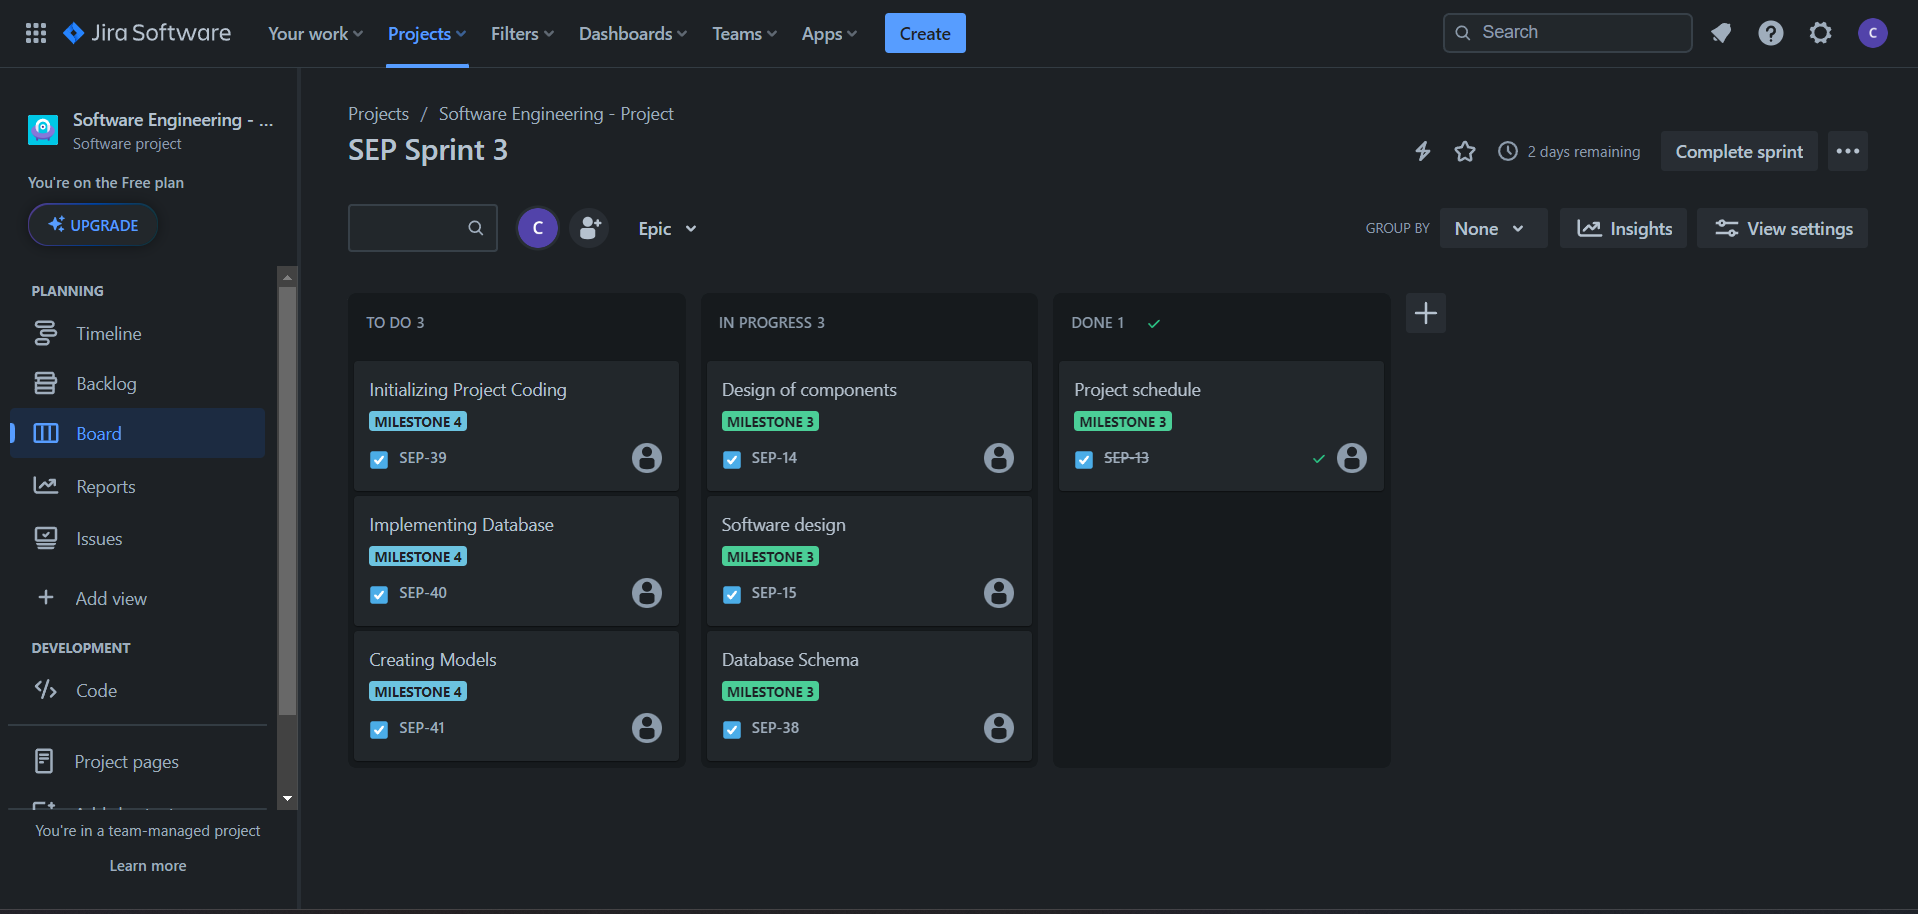
\includegraphics[width=1\textwidth]{img/PST.png}}
    \caption{Sprint Board in Jira}
    \label{fig:sprint_board}
\end{figure}

\subsection{Various Components}
\mysubsubsection{User Management Component}
    \begin{itemize}[label=\ding{212}]
        \tightlist
        \item Handles user authentication, registration, and profile creation.
        \item Assigns and manages user roles based on permissions.
        \item Provides user access control and permission management.
    \end{itemize}

\mysubsubsection{Profile Management Component}
    \begin{itemize}[label=\ding{212}]
        \tightlist
        \item Stores and retrieves user profile information securely.
        \item Manages user preferences, interests, and contact details.
        \item Enables profile updates and modifications by users.
        \item Ensures privacy and data protection measures for user profiles.
        \item Supports user-initiated data deletion or modification requests.
    \end{itemize}

\mysubsubsection{Course Management Component}
    \begin{itemize}[label=\ding{212}]
        \tightlist
        \item Adds, edits, and deletes courses from the catalog database.
        \item Manages course details such as name, description, instructors, and prerequisites.
        \item Controls the availability of courses for different terms or semesters.
        \item Handles updates and modifications to course information.
        \item Ensures data integrity and consistency within the course database.
    \end{itemize}
    
\mysubsubsection{Enrolment and Analytics Component}
    \begin{itemize}[label=\ding{212}]
        \tightlist
        \item Imports and exports enrolment data for analysis and recommendations.
        \item Generates statistical reports and insights for academic trends and performance.
        \item Tracks course popularity and student enrolment statistics.
    \end{itemize}
    
\mysubsubsection{Feedback and Rating Component}
    \begin{itemize}[label=\ding{212}]
        \tightlist
        \item Stores and manages student feedback and ratings for courses.
        \item Allows students to provide, edit or delete their feedback.
        \item Enables upvoting of helpful feedback from other students.
        \item Monitors and maintains the accuracy and relevance of feedback data.
        \item Facilitates analysis of feedback for course improvements.
    \end{itemize}

\mysubsubsection{Course Catalog Component}
    \begin{itemize}[label=\ding{212}]
        \tightlist
        \item Manages detailed information about available courses.
        \item Allows for sorting and filtering capabilities for users.
        \item Tracks and displays course availability and scheduling information.
        \item Maintains a comprehensive database of instructor details and feedback for each course.
    \end{itemize}
    
\mysubsubsection{Data Analysis Component}
    \begin{itemize}[label=\ding{212}]
        \tightlist
        \item Collects and processes statistical data for student performance.
        \item Conducts trend analysis for course popularity and academic patterns.
        \item Generates graphical representations and reports for data visualisation.
        \item Offers insights into academic progress and program assessment.
    \end{itemize}
    
\mysubsubsection{Recommendation Component}
    \begin{itemize}[label=\ding{212}]
        \tightlist
        \item Generates personalised course recommendations based on user profiles, completed courses, and interests.
        \item Utilises machine learning algorithms or rule-based systems for suggestion generation.
        \item Analyses user behaviour and preferences to suggest relevant courses.
        \item Collaborates with Enrolment and Analytics components to enhance recommendation accuracy.
    \end{itemize}

\subsection{Class Diagram}
A basic class diagram describing the application is given in \autoref{fig:class_diagram}. The diagram follows standard UML notations. The retuen type and parameters have been left empty for the classes, for the sake of readability.

There are 5 major Classes: 
\begin{enumerate}
    \tightlist
    \item User
    \item Recommender
    \item Feedback
    \item Course
    \item Analytics
\end{enumerate}
with their specializations as per given in the diagram. The dotted notation represents dependency of one component on another. This diagram shall be further modified to be in-line with flask framework to facilitate easy creation of APIs.

\begin{figure}[H]
    \centering
    \fbox{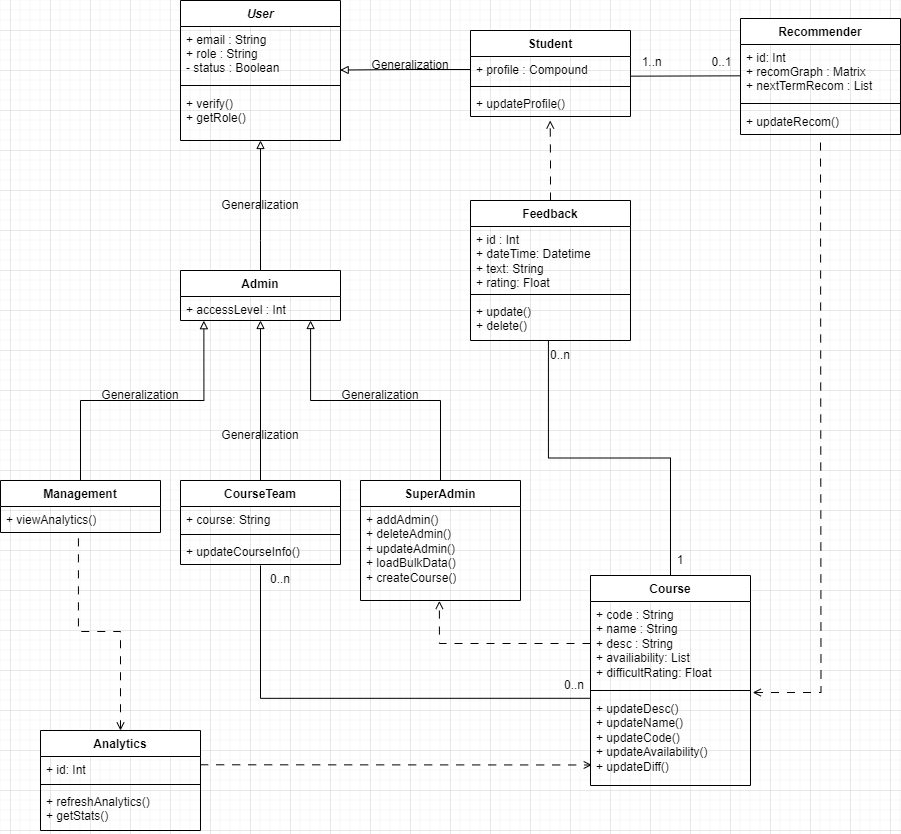
\includegraphics[width=1\textwidth]{img/class_diagram.png}}
    \caption{Basic Class Diagram}
    \label{fig:class_diagram}
\end{figure}
\vspace{1cm}

\subsection{SCRUM Meetings Schedule and Minutes}
Till date, 6 official meetings have been conducted details of which are in subsequent boxes. A lot of discussion also held via chat through WhatsApp. The major work completed, issues discussed and agenda is combined into a single heading "Minutes of the Meeting".

Meeting: Based on availability and need, after every 6 days starting from 2nd October.

\begin{myhbox}{2nd October, 2023}
    \begin{itemize}
        \item \textbf{Time}: 17:00 to 17:50 Hours
        \item \textbf{Duration}: 50 minutes
        \item \textbf{Who Attended}: Anchit, Anhat, Jasleen, Jay, Rohit
        \item \textbf{Agenda}: Introduction
        \vspace{0.5cm}
        \item \textbf{Minutes of the Meeting}: The main goal of the meeting was to introduce ourselves and to discuss basic approach to solve the given Problem Statement.
            \begin{enumerate}
                \item Introduced Ourselves
                \item Understood which tech-stack we are comfortable
                \item Identified main components in the projects:
                    \begin{enumerate}
                        \item Backend and Frontend
                        \item API
                        \item UI
                        \item Recommendation Algorithms
                    \end{enumerate}
                \item Understood and managed the timelines on Jira
            \end{enumerate}
    \end{itemize}
\end{myhbox}

\vspace{0.5cm}

\begin{myhbox}{8th October, 2023}
    \begin{itemize}
        \item \textbf{Time}: 19:00 to 19:29 Hours
        \item \textbf{Duration}: 29 minutes
        \item \textbf{Who Attended}: Anchit, Anhat, Jasleen, Jay, Rohit
        \item \textbf{Agenda}: Complete Sprint 1
        \vspace{0.5cm}
        \item \textbf{Minutes of the Meeting}:
            \begin{enumerate}
                \item Identified Primary, Seconday and Tertiary Users
                \item Understood SMART Guidelines
                \item Understood and wrote User Stories
            \end{enumerate}
    \end{itemize}
\end{myhbox}

\vspace{0.5cm}

\begin{myhbox}{15th October, 2023}
    \begin{itemize}
        \item \textbf{Time}: 16:45 to 17:15 Hours
        \item \textbf{Duration}: 30 minutes
        \item \textbf{Who Attended}: Anchit, Anhat, Jasleen, Jay, Rohit
        \item \textbf{Agenda}: Initialize discussion on Sprint 2
        \vspace{0.5cm}
        \item \textbf{Minutes of the Meeting}:
            \begin{enumerate}
                \item Wrote the important requirements for creating userboards
                \item Learnt and discussed different ways to create wireframes
            \end{enumerate}
    \end{itemize}
\end{myhbox}

\vspace{0.5cm}

\begin{myhbox}{18th October, 2023}
    \begin{itemize}
        \item \textbf{Time}: 20:35 to 21:09 Hours
        \item \textbf{Duration}: 24 minutes
        \item \textbf{Who Attended}: Anchit, Anhat, Jasleen, Jay, Rohit
        \item \textbf{Agenda}: Ensure uniformity in storyboard and wireframe design by each team member.
        \vspace{0.5cm}
        \item \textbf{Minutes of the Meeting}:
            \begin{enumerate}
                \item Initiated the work on creating a storyboard
                \item Created and discussed the essential wireframes
            \end{enumerate}
    \end{itemize}
\end{myhbox}

\vspace{0.5cm}

\begin{myhbox}{26th October, 2023}
    \begin{itemize}
        \item \textbf{Time}: 22:15 to 22:47 Hours
        \item \textbf{Duration}: 32 minutes
        \item \textbf{Who Attended}: Anchit, Anhat, Jasleen, Jay, Rohit
        \item \textbf{Agenda}: Complete Sprint 2
        \vspace{0.5cm}
        \item \textbf{Minutes of the Meeting}:
            \begin{enumerate}
                \item Completed all the wireframes
                \item Completed storyboards illustrating all the important features
            \end{enumerate}
    \end{itemize}
\end{myhbox}

\vspace{0.5cm}

\begin{myhbox}{1st November, 2023}
    \begin{itemize}
        \item \textbf{Time}: 16:05 to 16:27 Hours
        \item \textbf{Duration}: 32 minutes
        \item \textbf{Who Attended}: Anchit, Anhat, Jasleen, Jay, Rohit
        \item \textbf{Agenda}: Discuss Sprint 3
        \vspace{0.5cm}
        \item \textbf{Minutes of the Meeting}:
            \begin{enumerate}
                \item Created/Rectified Sprints and timings in JIRA
                \item Designed all the components diagrams
                \item Created a basic required class diagram
            \end{enumerate}
    \end{itemize}
\end{myhbox}